% 5-7 pages

% a.    Motivation
 
% c.    Analysis of strengths+weaknesses
 
% d.    Evaluation, including discussion of the lessons from the evaluation

\documentclass[letterpaper]{article}
\usepackage{aaai}
\usepackage{times}
\usepackage{helvet}
\usepackage{courier}
\setlength{\pdfpagewidth}{8.5in} 
\setlength{\pdfpageheight}{11in}
\usepackage{hyperref}
\usepackage{graphicx}
\usepackage{subfigure}
\usepackage{caption}
\graphicspath{ {images/} }


\title{Key Prediction and Chord Suggestions using Machine Learning and Case-Based Reasoning}
\author{Krishna Bathina \and Thomas Parmer}
\begin{document}
\maketitle

\begin{abstract}
    Technology is increasingly being used within the musical domain, in applications such as composition writing software, automatic accompaniment, electronic tuners, and music prediction. Here we build a system for novice music enthusiasts interested in composition. This system takes a list of chords as input, uses supervised machine learning to predict the most likely key signature for those chords, and then uses case based reasoning to find cases of similar chord progressions to compare with. The system then returns a suggestion of chords that the user can interact with.
\end{abstract}

\section{Introduction}

Music is of both great cultural and economic importance with large commercial interest in many applications of music classification and production, including thumbnailing, artist/song recognition, recommender systems, automated script reading, and computationally creative systems for music generation.  Computational creativity has shown promise in many domains, such as art and cooking \cite{elgammal2015quantifying,varshney2013big,ahn2011flavor,teng2012recipe}.  However, it is difficult to computationally create musical pieces for users due to the inherent complexity in categorizing music and understanding how musical styles and pieces relate to one another.  We attempt to make a system that does not replace the human composer but rather supplements the user's knowledge and creativity with chord suggestions based on domain knowledge of music theory.  This system is particularly useful for novice music enthusiasts with little theory background and can be used for composition, improvisation, and transposition between keys or instrumental parts.

Songs consist of notes and groups of notes (chords). Notes are represented as letters from A through G. In the simplest case, each note has 2 variants; a flat ($\flat$), or a half step lower, and a sharp ($\sharp$), or a half step higher. The notes and chords chosen in a song are not random but follow a pattern which comes from a song's \textit{key}, or group of pitches. Every note has many associated keys, the most common one made of 7 notes. $C, D, E, F, G, A, B$ is known as a $C$ major scale, or just $C$ scale. A major scale contains whole step intervals between all notes except the 2nd/3rd and the 6th/7th. This contrasts with a minor scale, in which the 3rd, the 6th, and the 7th are all one half step lower than in the major scale. For example, a $C$ minor scale ($Cm$) contains $C, D, E\flat, F, G, A\flat$, and $B\flat$. 

Another popular scale is the 12 note chromatic scale, shown in Figure~\ref{chromatic}. Each note is a half step apart from the previous note. Another common convention is to assign $C$ to 0 and $B$ to 11. This allows for convenient mathematical operations to be done modulo 12.

In popular music, many songs are chord-based with common chords being the major chord (containing the first, third, and fifth notes of the scale), and the minor chord (containing the first, flat third, and fifth notes of the scale).  Associated with each key is a diatonic chord progression, composed of chords that contain notes naturally found within the scale.  The diatonic progression for a major scale is the major root, a minor second, a minor third, a major fourth, a major fifth, a minor sixth, and a diminished seventh.  If the root chord is minor, then the progression is a minor root, a diminished second, a major third, a minor fourth, a minor fifth, a major sixth, and a major seventh.  The sixth of a major key is the minor key with the same scale and vice versa.

\begin{figure}[ht]
	\centering
	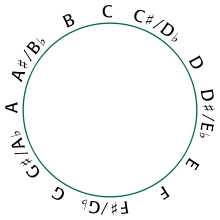
\includegraphics[width = 0.5\columnwidth]{chromatic.png}
	\caption{Every note in the chromatic scale.}
	\label{chromatic} 
\end{figure} 

The use of computer science and machine learning in music is an increasingly popular topic. \cite{dubnov2003using}, for example, analyzes MIDI files and predicts what to play next by dividing the song into motifs and analyzing each one. A more intricate predictor from~\cite{ni2012end} applies short time Fourier transformation along with other complicated spectral analyses to estimate key sequences and bass notes. \cite{dhanaraj2005automatic} used acoustic features as well as lyric-based features in order to predict the popularity of a song and \cite{eck2007autotagging} did similar work to generate genre tags.  \cite{mauch2015evolution} used features from the Million Song Dataset to show that there have been several stylistic revolutions during the evolution of recent popular music.  Another study used a convolutional deep belief network for key detection, along with genre and artist recognition \cite{Dieleman}.  Other work has looked at year prediction, thumbnailing, cover song prediction, and evolution of musical dimensions in popular music \cite{Foster3,Chai,Foster2,Serra}.

Case-based reasoning also has many applications in music. Sicom uses temporal case-nodes to represent cases for music composition~\cite{pereira1997composing}. Each case node is a specific time point in the song with some basic features. Suggestions are made by searching for case nodes with similar features. Another system, SaxEx (Saxophone Expressivism), uses simple case-based reasoning with analysis of sound files to generate expressive music~\cite{arcos1998saxex,arcos2001interactive,de2012playing}. Written in Noos, the system takes the score of the piece and a MIDI file of the inexpressive phrases. They are then analyzed using Spectral Modeling Synthesis (SMS). The analysis is used to find similar cases using a majority-wins rule for matching. The suggestion is then adapted to the input using SMS, and a MIDI file of the express phrase is outputted. 

In this paper, we make a system where novice users with minimal understanding of music theory can input a set of chords and get a recommendation of other chords to play next. This system includes both traditional machine learning and case based reasoning. This is an important task for two main reasons: it combines two common artificial intelligence approaches and is usable even to naive users.

\section{Data}
We use two datasets to build and validate our model. The first was built from scraping \href{https://www.ultimate-guitar.com/}{UltimateGuitar.com}. UltimateGuitar is a database of user-submitted transcriptions for songs. When searching for a song, a user can choose amongst of list of transcriptions ranked by popularity. In total, our dataset contains about 100,000 songs and its chords. In order to find the key, we matched our dataset with the \href{https://labrosa.ee.columbia.edu/millionsong/}{ Million Song Dataset}~\cite{bertin2011million}. This dataset (MSD) was produced from LabRosA at Columbia University, and contains metadata for each song, including song name, artist name, genre terms, and key.  In order to match songs between the two datasets, we converted the artist and song names to a standard format by removing spaces, punctuation, and reformatting words that are commonly written in different ways (e.g. 'featuring', 'feat', 'ft').  We kept only songs where both the standardized song name and artist name matched.  We  also threw out songs that did not have a valid chord progression.  We consider only major and minor chords here; in cases where we could, we transformed augmented chords to their base value (\textit{e.g}, we changed $G7$ to $G$ or $Fm13$ to $Fm$).

The resulting filtered dataset contains 13,477 songs. A histogram of the genres and the keys of the songs are shown in Figure~\ref{data}. The most common genre is Alternative \& Punk and the least common is Classical. This makes sense because UltimateGuitar.com contains transcriptions for guitar and bass. The most common keys match the top keys from the most popular songs on Spotify ($G, C, D, A, C\sharp, F$)~\cite{spotify}.

\begin{figure}[t]
	\centering
	\subfigure{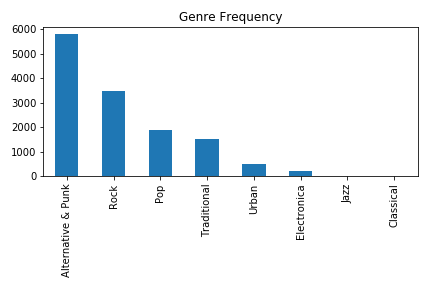
\includegraphics[width = \columnwidth]{genre.png}}
    \subfigure{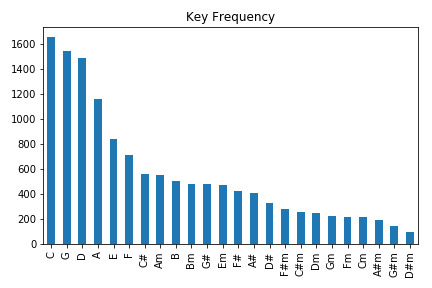
\includegraphics[width = \columnwidth]{key.png}}
	\label{during}
	\caption{The figure on the top shows the genre frequency while the below shows the key frequency.}
	\label{data} 
\end{figure} 

\begin{figure}[t]
	\centering
	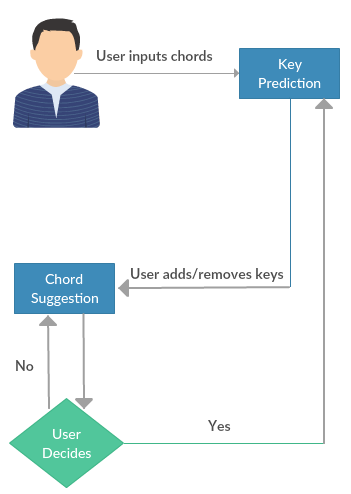
\includegraphics[width = \columnwidth]{flowchart.png}
	\caption{The flowchart represents how the user interacts with our system.}
	\label{flowchart} 
\end{figure} 

\section{Methods}
\subsection{System}

Our system first accepts a list of chords from the user. The chords are then quality-checked and passed to the key suggestion module. Using supervised machine learning, the module returns a list of possible keys. The user can choose to remove any of the keys and add any they want to. Afterwards, the keys are passed to the chord suggestion module. This uses case-based reasoning to find similar and creative suggestions based on songs in the database. The suggestions are returned as a chromatic position from [0-11]. Each suggestion is then converted to their associated chord in the chromatic scale. Because each position can refer to multiple chords ($C\sharp, D\flat$), the system chooses the chord the appears most frequently in the list of possible keys. Afterwards, the chords are presented to the user one at a time. If the user rejects the chord, the next ranked chord is presented. On the other hand, if the user accepts the chord, the process is restarted from the key prediction module with the new chord added to the user input. A flowchart of the system is shown in Figure~\ref{flowchart}.


\subsection{Key Prediction}
We used supervised learning in order to predict the key from a sequence of chords.  In order to create a good classifier, we tried various learning tasks, including predicting whether a chord progression belongs to a major or minor key, what specific key a chord progression belongs to, and whether to accept or reject a given key based on the distribution of chords relative to that key.

Our main goal was to predict which key each song belonged to, where our feature list was derived from the chords in the Ultimate  Guitar dataset and the label (key) came from the Million Song Dataset.  There are 24 possible keys (considering 12 unique chromatic positions that each have a major and a minor variety).  Our baseline for comparison was predicting the chord that appeared the most within the song to be the correct key.  

We then considered using a feature vector based on the normalized frequencies of each chord out of the 24 possible unique chords; however, this approach is still naive as it uses simple frequencies rather than musical domain knowledge.  In an attempt to incorporate musical theory into our machine learning, we also tested learning on features derived from relative chords; that is, instead of our feature vector holding frequencies for [$C....B,Cm...Bm$], it held frequencies for [Root,flat Second, Second, flat Third, Third....,Minor Root, Minor flat Second...Minor Flat Root].  Because many songs use diatonic chord progressions, we assumed that key could be discovered by looking at the distribution relative to the root.  Common distributions, for example, would have spikes at the first, the fourth, and the fifth, while having low frequencies for uncommon chords, like the flat second or the flat fifth.  Figures~\ref{major_average} and \ref{minor_average} show the average frequencies of the relative chord positions for each song in our dataset; the diatonic chords are shown in red for major and minor scales respectively.  These distributions confirm that diatonic chords are more common than random chance alone would dictate.

\begin{figure}
	\centering
	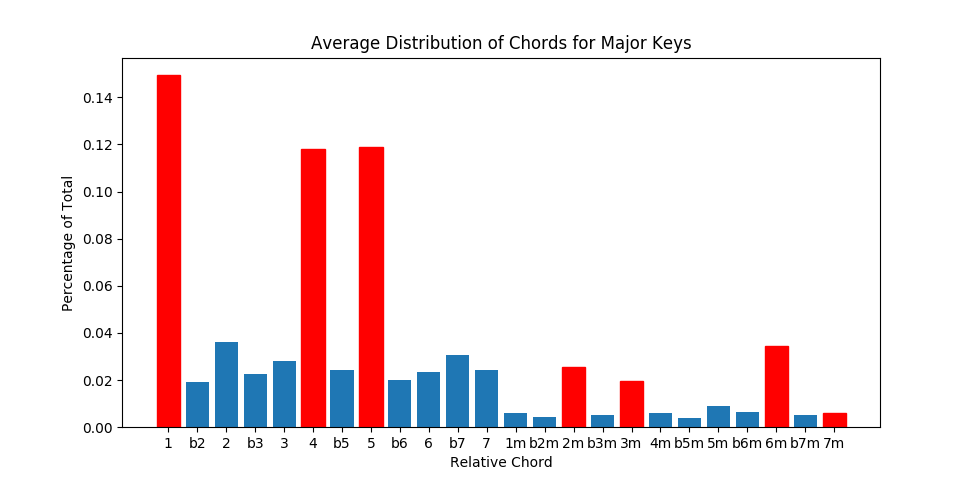
\includegraphics[width = \columnwidth]{major_average_dist.png}
	\caption{Distribution of relative chords for songs with a major key.  Chords from the major diatonic chord progression are shown in red.  Note that the diminished 7th is considered minor here for simplification.}
	\label{major_average} 
\end{figure}

\begin{figure}
	\centering
	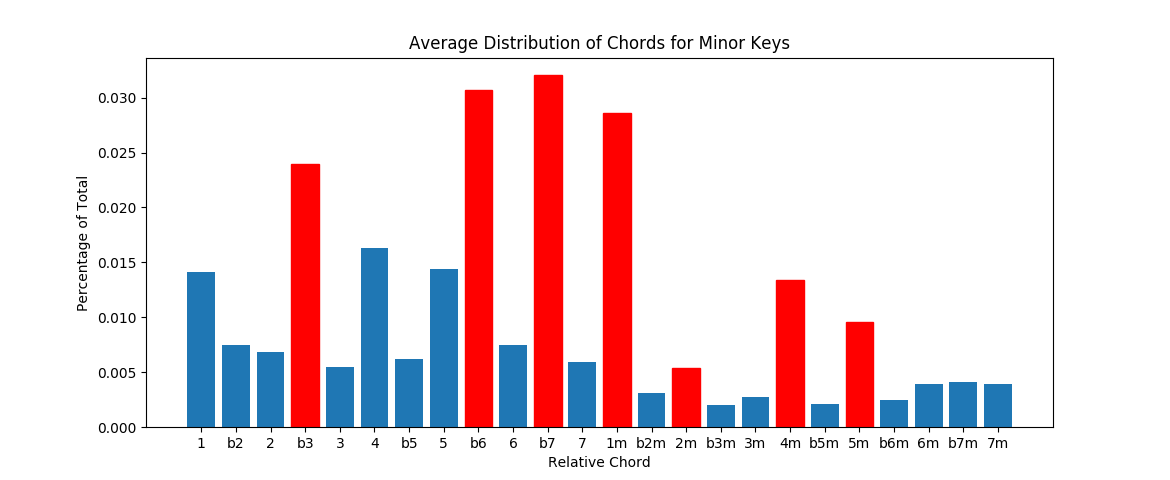
\includegraphics[width = \columnwidth]{minor_average_dist.png}
	\caption{Distribution of relative chords for songs with a minor key.  Chords from the minor diatonic chord progression are shown in red.  Note that the diminished 2nd is considered minor here for simplification}
	\label{minor_average} 
\end{figure}

However, it is impossible to build a relative chord distribution without knowing what the root chord is, which would imply that the key is already known \textit{a priori}.  To make a practical system, we therefore generated a relative distribution for every chord from each song in the testing set and labeled it as either positive (it was the true key) or negative (it was not the true key).  Then, we tested chords from each song in the testing set and assigned confidence scores based on how likely that chord was the correct key based on its relative chord distribution.  We then chose the chord with the highest score as our label prediction.  We tested both the subset of chords found in the song and all 24 keys.  Although it is unlikely that a song would not contain its root chord, this is likely to occur if a user gives the system only a few chords and the system needs to recognize the key based on this small amount of information.  We also learned a classifier where features were based on the difference between the relative normalized  frequencies of the chords and the average distributions shown in Figures~\ref{major_average} and \ref{minor_average}.

For the relative distribution tasks, we tested the difference between using a single classifier and using a separate classifier for major and minor modes.  We also tried using a two-part classification, where first we ran a classifier to determine if the song was likely in a major or minor mode and then used these results to filter the keys that we were considering; afterwards, we ran the regular relative classifier.  Finally, we tested the combination of using both an absolute classifier and a relative classifier to combine the natural frequencies present with music theory knowledge of common chord progressions.  We tried two different methods for combination: finding the rankproduct and finding the product of the absolute and relative confidence scores.  We present the top five results to the user for verification, provided that the key's score is above zero.

For each classification task, we used a Support Vector Machine (SVM) from Python's scikit-learn module \cite{scikit-learn}.  We used grid search to determine the best parameter settings and compared performance to decision trees.  In addition to using normalized chord frequencies, we experimented with adding additional features for the first and last chord in a song because many songs either start or resolve on their root chord.  For a full description of what experiments we ran, see the comments in classify\_kb.py.


\subsection{Chord Suggestion}

Typical case-based reasoning uses a similarity metric in order to find cases. In our system we use key and pattern matching as a similarity measure. We separate our selected cases into two groups: similar and creative. To find similar cases, we subset the data into all songs with the suggested keys. We then search through the subset for the exact same chord progression inputted by the user. The suggestions are thus the next chords in each song.

We gathered the creative cases by first finding the complement of the similar subset. We then take the songs and the user-inputted chord and convert then into a chromatic scale. For example, a song with with the chords [$D, F\sharp, A, B$] would be converted to [2, 6, 9, 11]. Instead of searching for the exact chord progression, we search for songs with the same pitch difference. In our example, [2, 6, 9, 11] would be represented by the difference in pitches as [4, 3, 2]. If the user-inputted chords are [4, 3], the suggestion would be 11. The creativity from this part comes from the fact that we are matching by the differences in pitches and not the actual pitch itself. For example, both $C$ to $D$ and $E$ to $F\sharp$ would be considered equivalent. 

The user is asked to input a creativity factor from [0,1].
For both similar and creative cases, the proportion of each suggestion is calculated. The creative suggestions are scaled by the creativity factor and the similar suggestions are scaled by 1 minus the creativity factor. The combined proportion is then calculated as the average of the two as shown in Equation~\ref{cbr}. The chords are then chosen randomly with probability equal to their scaled proportions and then passed to the user.

\begin{equation}
P(S_i) = \frac{(1-C)*SProp(S_i)
+ C*CProp(S_i)}{2}
\label{cbr}
\end{equation}


\section{Evaluation}
\subsection{Key Prediction}

The baseline performance of predicting the most frequent chord as the key was 25\%.  Performance in key prediction across the other classifiers was similar and around 40\%, regardless of whether absolute or relative chord distributions were being used.  This suggests that the amount of knowledge that we gain from musical theory is roughly equivalent to the amount of knowledge embedded in chromatic frequencies, in these tasks.  Both types of knowledge outperform baseline performance.

Absolute chords distributions inherently test all possible chromatic positions and thus they were not tested with only the chords in the song, nor could the difference from the average normalized major\/minor distributions be calculated.  Nevertheless, they obtain around 40\% accuracy when testing against all possible chords.  Relative chords do very poorly at this task because they cannot differentiate between major and minor modes.  However, if you use a separate classifier for each mode, then performance of the relative chords increases to 40\% as well.  Using relative chords from the song only also achieves this performance.  Interestingly, adding the first and last chord as features increases accuracy when considering a single relative classifier but decreases accuracy when using a separate relative classifier for each mode.  Two-part classification and combining absolute and relative classifier scores also performed similarly.  Adding a separate modal classifier boosted accuracy when combining absolute and relative classifiers, and the highest performance when considering either the chords in the song or all 24 chromatic chords occurs by choosing the key with the highest product of absolute and relative confidence scores using modal relative classifiers.

One task where domain knowledge helps rather than using absolute chord frequencies is predicting a chord sequence as either major or minor.  Accuracy in major\/minor classification is around 8\% higher when using relative positions and gives an accuracy of 84\% when considering the first and last relative chords as features.

In our system, we need to consider circumstances where the user only inputs a few chords.  Therefore, it is quite likely that the proper key is not in the user's input and so we want to consider all chromatic positions when making our determination.  We also don't want to rely on the identity of the first or last chord since the chord progression is modified online.  The highest performance matching these conditions (and the highest overall) was to implement a combination of absolute and relative modal classifiers.  This is what we use in our system to generate our key predictions.  However, because accuracy is rather low (42\%), we present the user with our top five choices as long as there are five choice with a confidence score above 0\%.

\begin{table*}[t]
\centering
\caption{Results from Key Prediction on UltimateGuitar data.  With a few exceptions, performance across classifiers is very similar, whether using absolute or relative chord frequencies.  The best performance comes from the product of absolute and relative classifiers while using separate classifiers for major and minor modes.}
\label{my-label}
\begin{tabular}{lcccc}
Task & Major/Minor &  Key from chords in song &  Key from all chords \\ \hline   
Most Freq                               & N/A                 & 0.2509                                                                        & N/A                                      \\
Absolute Norm. Chords                                             & 0.753               & N/A                                                                           & 0.4016                               \\
ABS with F/L                                                      & 0.7637              & N/A                                                                           & 0.3915  \\
Relative Norm. Chords                                             & 0.8312              & 0.3856                                                                        & 0.0438   \\
REL with F/L                                                      & 0.8412              & 0.4105                                                                        & 0.0501  \\
Mode Separate                                                     & N/A                 & 0.3971                                                                        & 0.3911\\
Mode with F/L                                                     & N/A                 & 0.3515                                                                        & 0.3348 \\
2-part Classification                                             & N/A                 & 0.3852                                                                        & 0.366 \\
Rankproduct of ABS * REL                                          & N/A                 & 0.3856                                                                        & 0.3808  \\
Rankproduct w/ Mode & N/A                 & 0.4116                                                                        & 0.4042 \\
Product of ABS * REL  & N/A                 & 0.3886                                                                        & 0.3793 \\
Product with Mode     & N/A                 & 0.4175                                                                        & 0.4156                                 
\end{tabular}
\end{table*}


\subsection{Chord Suggestion}

Evaluating chord suggestions is very difficult because there is no measure that can determine if a chord belongs in a piece. Key signatures and common patterns can be used as templates, but do not dictate the correctness of a chord. This is all decided by the artist. Instead, we followed the evaluation guidelines of Klaus-Dieter Althoff in \textit{Evaluating case-based reasoning systems}~\cite{althoff1995evaluating}. His evaluation consists of three parts: technological, ergonomic, and domain. 

The technological criteria focuses on 5 implementation details. \textbf{Knowledge Representation}: Our database consists of songs, keys, and chords. Because our system is meant for naive users, we don't include more complicated features such as the MIDI file. \textbf{Organization of Case Library}: Our cases are stored in a Pandas DataFrame. \textbf{Similarity Assessment}: In our system, similarity is measured by key rather than by song (case). \textbf{Noisy and Incomplete Data}: Because the input is a list of chords, noisy chords and incomplete phrases are impossible to filter automatically. But, the user does have the ability to remove incorrect chords. \textbf{Performance}: Because of a static database, our data structure allows for searching and indexing in linear time.

The ergonomic criteria is centered around 5 details about usability.\textbf{Control of Application Development}: Because there were only two people working on the system, there were no issues with application development. \textbf{Validation and Testing}. We validated and test our model by manually matching cases and by testing how well the creativity factor actually produced novel suggestions. \textbf{Acquisition and Maintenance of Knowledge}: Because we do not add new cases or modify existing cases, there is no maintenance needed after the initial cleaning. \textbf{Explainability}: Our system does not directly explain the logic of each individual suggestion but instead for all suggestions at once. \textbf{User Acceptance}: While we have not yet tested our system with a third party user, we believe it will be accepted because of its clear instructions and ease of use. 

The domain criteria consists of many details, of which we focus on 6. \textbf{Size}: Our database consists of about 13,000 songs. \textbf{Complexity}: The only relationship between the cases are the keys. But, when searching for suggestions with pattern matching, there is also a relationship with the user-inputted chords. \textbf{Theory Strength}: Most of the feature engineering came from ourselves. \textbf{Neighborhood Notion}: There is no sense of similarity between cases besides similar keys. \textbf{Reasoning Strategy}: Our reasoning strategy initially is side by side -- each song is analyzed separately. When deciding on the suggestion, the reasoning style switches to majority rule.

\section{Discussion}

Our system is different from typical chord suggestion systems because it first makes predictions about the key signature and then uses case based reasoning to suggest the next chord. The key signature allows us to apply domain knowledge about musical theory to the chord progression, and it allows us to find similar songs in the case base depending on the particular key.  We use a large case base of thousands of songs and a creativity parameter to suggest novel, but feasible, chords to the user.  This allows for some computational 'creativity' to aid the user in making their next chord choice. We decided not to add new cases to our database because many songs that a user comes up with will be fragmentary or undeveloped, and we want to ensure high quality control of our case base.

An additional advantage to our system is that it runs quickly and does not require very much memory.  Because our database is of constant size, the system is almost constant time through searching. Adding through the database will increase the search time linearly in the number of cases.  Our classifier models are pre-built so classification is done in polynomial time in the number of chords using an RBF kernel.  As such, our system would be easy to scale to longer inputs or multiple users.

There are many issues that we have not fully addressed in our system. First of all, the UltimateGuitar.com dataset is meant for guitarists and bassists. Thus many of the songs in the original dataset are transposed form their original version. As noted by the users, some of the songs were purposefully transposed into another key. Also, because UltimateGuitar.com is meant for music enthusiasts, the verification for uploaded songs is by popularity, not expert knowledge.  This noise in our dataset affected both the accuracy of our classifiers as well as the accuracy of the cases in our case base.

Accuracy in our key prediction tasks is also lower than what would be ideal for a commercial system.  Key prediction is inherently difficult in this domain because there are 12 possible chromatic chords in both major and minor modes, resulting in 24 labels for our data.  Although diatonic chord progressions can be used as a guideline, they are not strict rules which musicians follow during composition.  There is also overlap between different keys so it can be difficult to tell similar keys apart from one another.  Finally, both key prediction and our case retrieval is limited by the amount of data that we get from the user.  Our system may need to make suggestions based on only three or four chords that the user inputs.

There is much further work that can be done with this idea. The user interface can be modified so that a user can input their own chord and see how it changes the key prediction. The key prediction classifier can also be built by using natural language processing and n-gram techniques to extract patterns of repeated notes (\textit{i.e.} musical phrases). The case based reasoning can also be improved by being more strict with the similar cases. Similar cases can be ranked amongst themselves, thus giving a more specific ranking for the suggested chords. 

Our system is expandable to many other fields. With more advanced techniques for example, the system can be used for synonym suggestion. Many times when asking for synonyms, a replacement with the same definition but different connotation is given (e.g. 'smile' and 'smirk'). By looking at similar cases (uses of the word in various definitions), a similar system will be able to suggest a connotatively better synonym. With careful feature selection, this can also be used for word, fragment, and sentence suggestions. 

\bigskip
Krishna worked with the UltimateGuitar dataset and Thomas worked with the Million Song Dataset. Krishna did much of the work on CBR, while Thomas did much of the work on the machine learning.  They both worked on the analysis, the paper writeup, and the presentation.

All of our code can be found online at https://github.com/kbathina/Music-KB-AI.  

\bibliography{bib}
\bibliographystyle{aaai}

\section{Screenshots}
\begin{figure}[t]
	\centering
	\subfigure{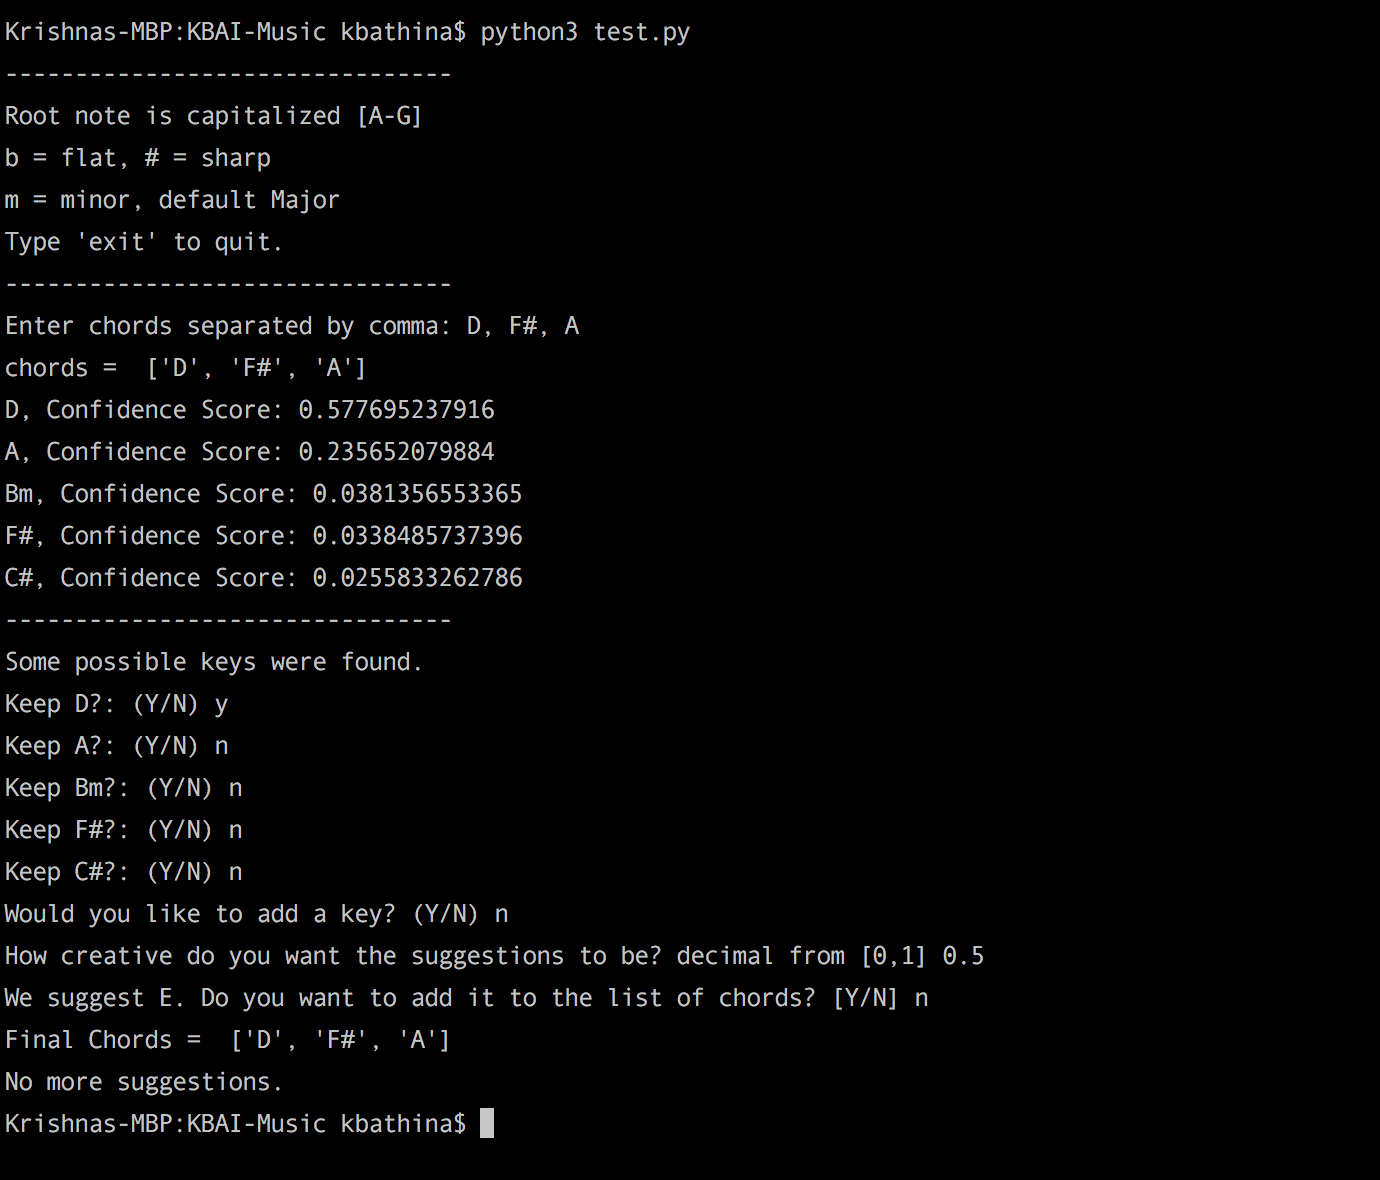
\includegraphics[width = \columnwidth]{1.png}}
    \subfigure{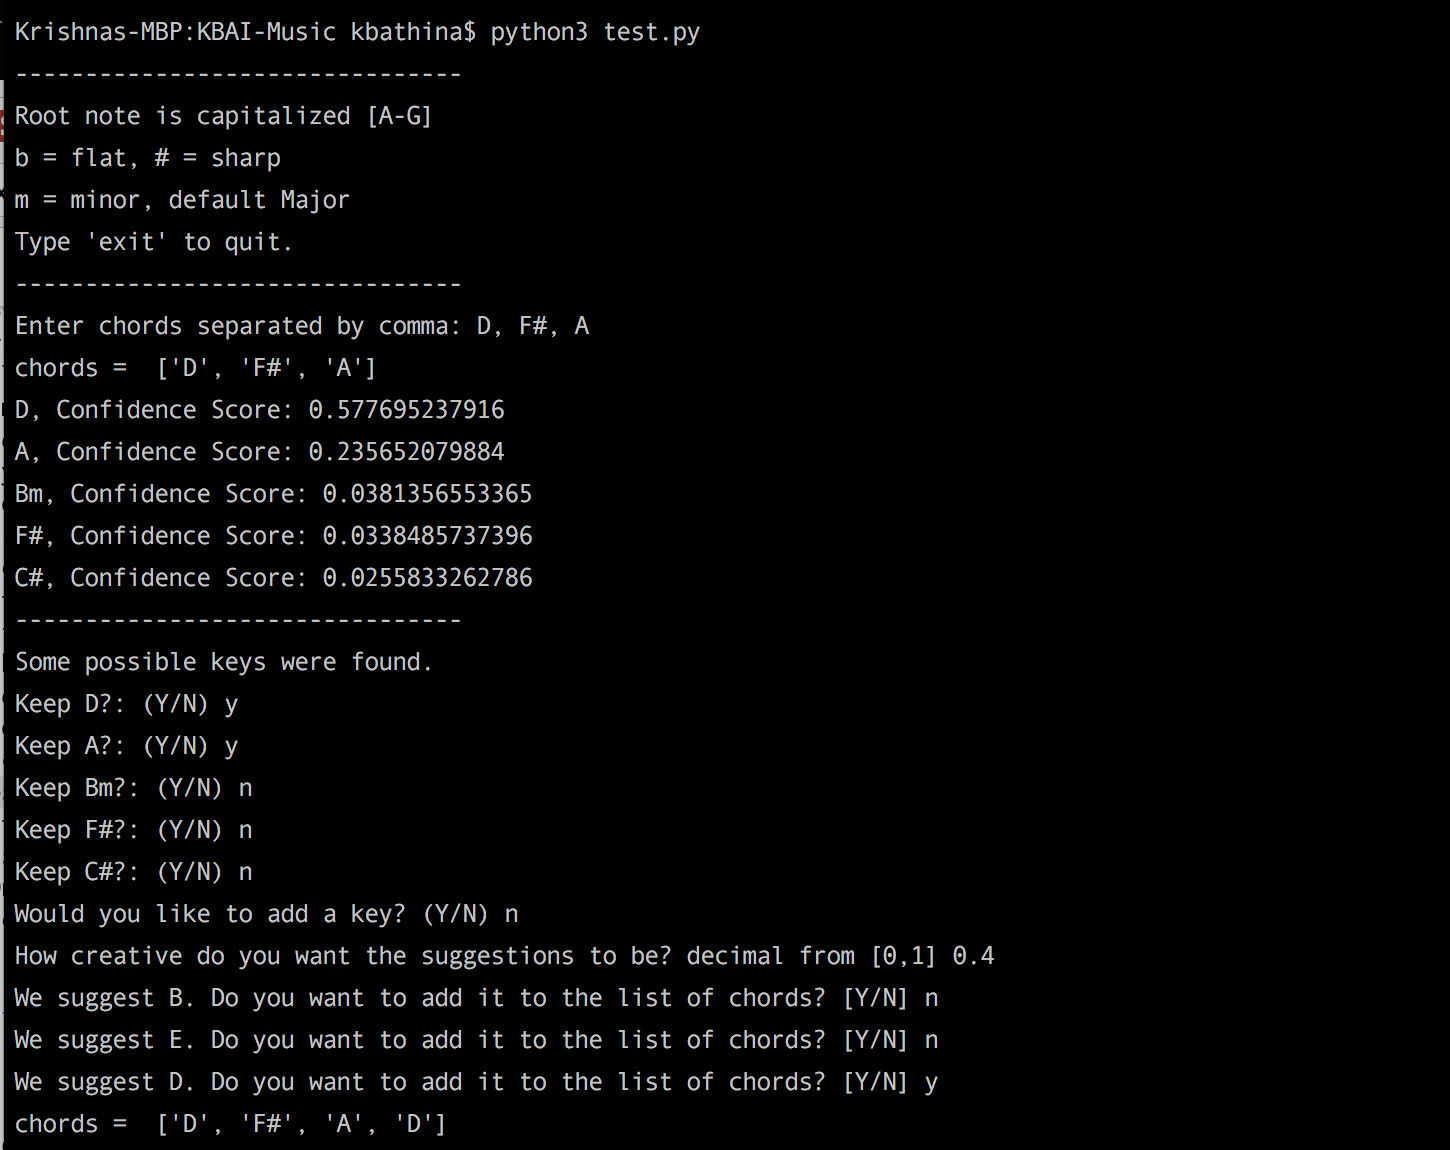
\includegraphics[width = \columnwidth]{2.png}}
    \subfigure{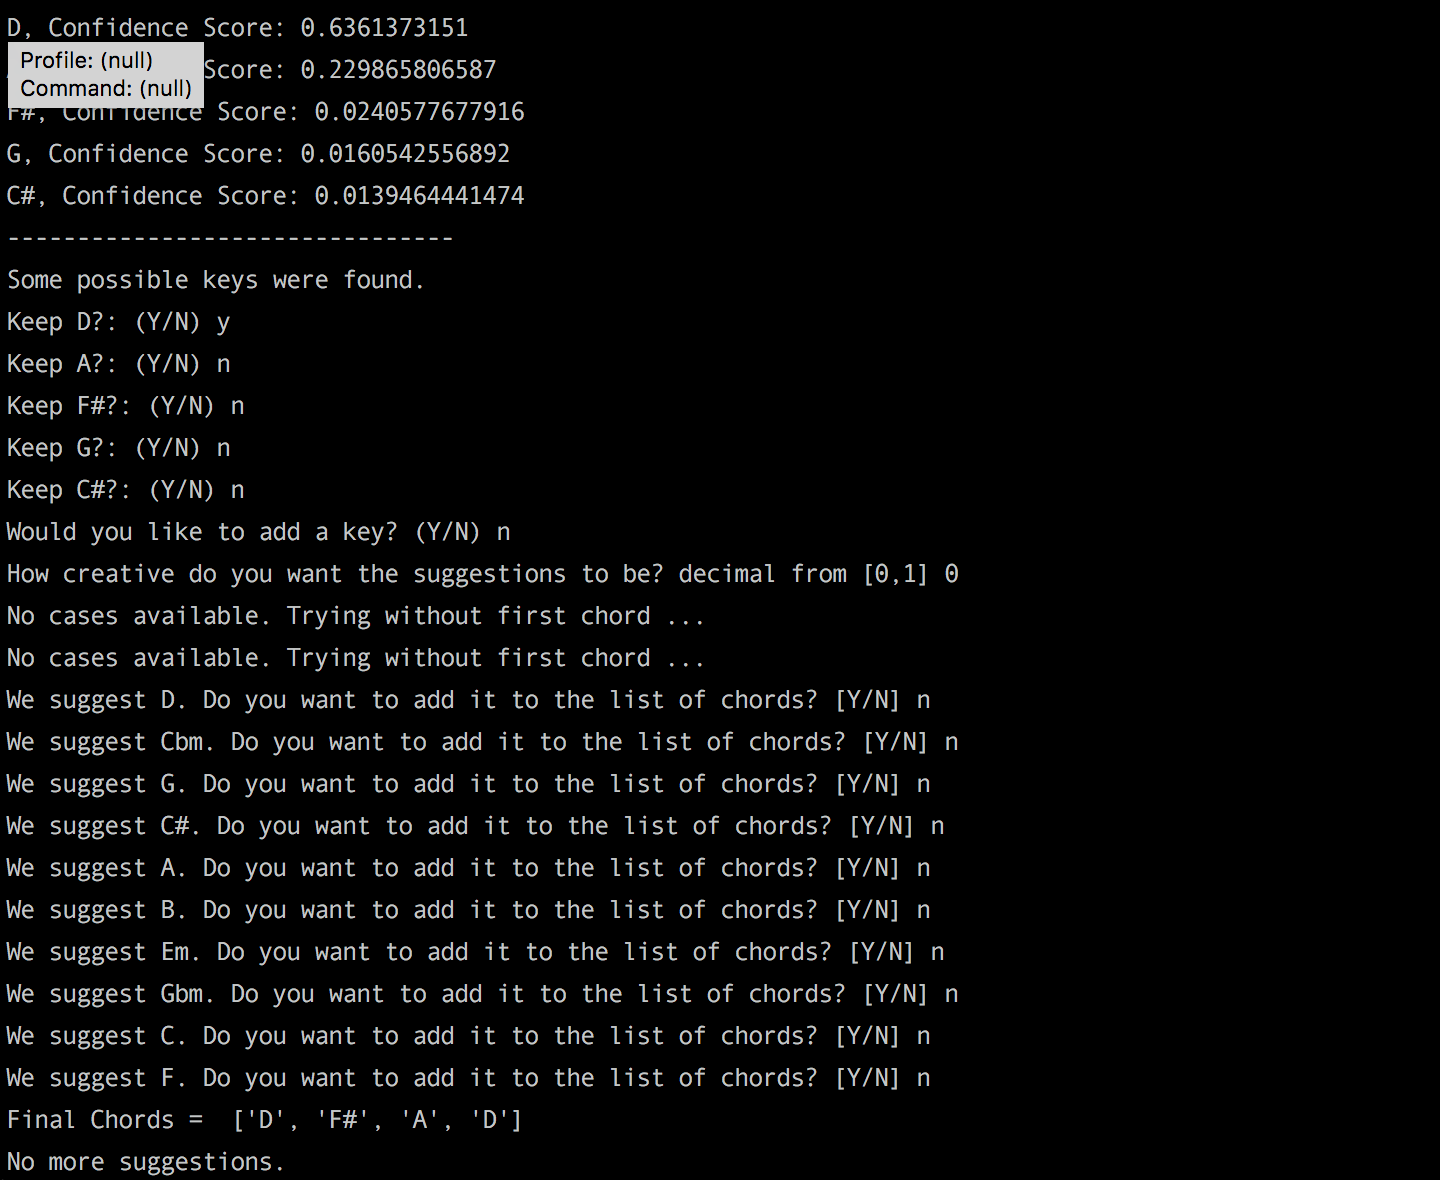
\includegraphics[width = \columnwidth]{3.png}}
	\caption{Screenshots of some sample runs of our system.}
	\label{screenshot} 
\end{figure} 
\end{document}